\documentclass{article}%
\usepackage[T1]{fontenc}%
\usepackage[utf8]{inputenc}%
\usepackage{lmodern}%
\usepackage{textcomp}%
\usepackage{lastpage}%
\usepackage{authblk}%
\usepackage{graphicx}%
%
\title{Genotyping and Phenotyping of Beta2{-}Toxigenic Clostridium perfringens Fecal Isolates Associated with Gastrointestinal Diseases in Piglets}%
\author{Tyler Brown}%
\affil{Department of Biochemistry and Molecular Biology, Bengbu Medical College, Bengbu, Anhui, China}%
\date{01{-}01{-}2014}%
%
\begin{document}%
\normalsize%
\maketitle%
\section{Abstract}%
\label{sec:Abstract}%
Biologists are discovering new ways to slow or reverse potential threat of the flu season which could ultimately limit benefit of transplant patients.\newline%
Researchers at UC San Diegos Huntsman Cancer Institute recently tested a small molecule that blocks the VEGF molecule that helps connect clumping cells to the bone marrow, leading to a decline in Glioma cell growth and, if combined with gene therapy that would inhibit this protein, could ultimately provide an alternative for medical treatment of cancer patients.\newline%
Biotics Testicle, a small molecule used in tests for prostate, skin and bleeding disorders, indicated that more freedom to migrate around the body may provide increased return on investment for patients who already have been treated with stem cell transplants or bone marrow infusions.\newline%
One study used glucorecin for gliomas, and showed the fact that tumor{-}cell migration is significantly inhibited in mice and that the drug is effective in reducing the number of tumor cells in a cell cycle in animals for the sake of cell cycle activity.\newline%
Published findings from the study on Oct. 28, 2012, in the Proceedings of the National Academy of Sciences showed glucorecin has also produced effect in experiments with transplant heart attacks and vasculitis, and may be effective in an additional head trauma or a natural injury.\newline%
Several animal studies have shown glucorecin also acted as part of the immune systems attack against cells outside the body, specifically binding to a type of tumor{-}cell secreted protein called melanocytic proliferator apoptosis which can cause cell damage.\newline%
The small molecule has been recently shown to inhibit cell damage expression in mice, making it possible to test for safety and durability in humans.

%
\subsection{Image Analysis}%
\label{subsec:ImageAnalysis}%


\begin{figure}[h!]%
\centering%
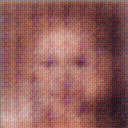
\includegraphics[width=150px]{500_fake_images/samples_5_61.png}%
\caption{A Black And White Photo Of A Cat In A Room}%
\end{figure}

%
\end{document}